\section{问题一：基于常物性闭合的预热平衡阶段模型}
\label{sec:p1}

\subsection{物性闭合与输运尺度判别}

问题一取附录 2 的物性：密度 $\rho=820$ kg/m$^3$、比热容 $c_p=2600$ J/(kg·K)、
热传导系数 $k=0.36$ W/(m·K) 三者均为常数，只有水分扩散系数依赖含水率，

\begin{equation}
D(C)=7\times10^{-9}\,\mathrm{e}^{-0.89/C}\quad\text{m}^2/\text{s}.
\label{eq:D_app2}
\end{equation}

半径固定为 $R_0=0.02$ m。于是式~\eqref{eq:heat_s}~的系数全为常数、
温度方程成为线性方程，而式~\eqref{eq:mass_s}~仍因 $D(C)$ 而非线性。
这一非对称性是问题一独有的机会：温度场可以另求解析解，
从而构造一条不依赖本文离散格式的校验通道。

热扩散率

\begin{equation}
\alpha=\frac{k}{\rho c_p}=\frac{0.36}{820\times2600}
=1.6886\times10^{-7}\quad\text{m}^2/\text{s},
\label{eq:alpha}
\end{equation}

预热段终点的热 Fourier 数 $\mathrm{Fo}=\alpha t/R_0^2=0.759850$，量级为 $1$，
说明 $1800$ s 恰好是热扰动穿透半径所需的时间尺度。水分一侧，初始含水率下
$D(2.55)=4.937\times10^{-9}$ m$^2$/s，比 $\alpha$ 小 $34.2$ 倍，
质 Fourier 数仅 $0.0222$。扩散长度按 $\sqrt{Dt}$ 缩放，
两者相差 $\sqrt{34.2}\approx5.85$ 倍，即同样时间内湿分扰动只能推进热扰动
约六分之一的距离。再配合 $Bi=1.3889$ 与 $Bi_m=3.24$，可对本阶段的输运结构作出主要尺度判断：
热一侧 $Bi$ 为 $O(1)$，内外热阻相当，表面既非等温也非绝热；
质一侧 $Bi_m=3.24$ 明显大于 $1$ 且约为 $Bi$ 的 $2.3$ 倍，
表面对流不是控制环节，内部扩散阻力才是，这与湿分只在薄壳内变化的结果一致。
两侧的推进速度相差近六倍。这四个数各自只在其定义的机制上有效，
给出的是量级判断，不替代耦合方程的完整求解。

\subsection{完整模型}

问题一的完整模型为式~\eqref{eq:heat_s}~与~\eqref{eq:mass_s}~取 $R\equiv R_0$，

\begin{align}
\rho c_p\frac{\partial T}{\partial t}
&=\frac{4k}{R_0^{2}}\frac{\partial}{\partial s}
\left(s\frac{\partial T}{\partial s}\right),
\label{eq:p1_heat}\\
\frac{\partial C}{\partial t}
&=\frac{4}{R_0^{2}}\frac{\partial}{\partial s}
\left(s\,D(C)\frac{\partial C}{\partial s}\right),
\label{eq:p1_mass}
\end{align}

配以式~\eqref{eq:bc_s}~的表面 Robin 条件、式~\eqref{eq:D_app2}~的扩散系数闭合
与题给均匀初值 $T=28$ °C、$C=2.55$ kg/kg，时间区间 $[0,1800]$ s，
其中 $T_{\mathrm{air}}$、$W_{\mathrm{air}}$ 由附件 1 插值。
按第~\ref{sec:model}~节的格式取 $N=160$、$\Delta t=0.25$ s 推进求解。

\subsection{结果与制表}

\begin{figure}[!htbp]
  \centering
  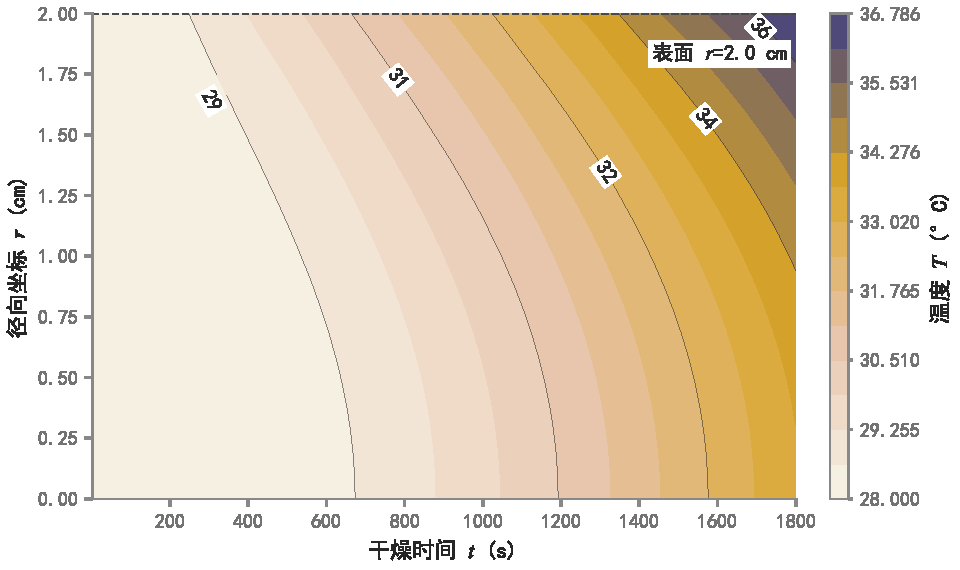
\includegraphics[width=0.9\textwidth,height=0.8\textheight,keepaspectratio]{../figures/fig_q1_field_T.pdf}
  \caption{问题一温度场分布}
  \label{fig:q1_field_T}
\end{figure}

图~\ref{fig:q1_field_T}~的等温线自表面向中心平移，前 $300$ s 内几乎贴着表面，
此后逐步深入。$1800$ s 时表面温度 $36.7857$ °C、中心 $33.5757$ °C，
内外温差 $3.2100$ °C，尚未抹平；同期热风为 $41.513$ °C，
表面仍比热风低 $4.7$ °C。三个数字共同说明预热段结束时药材既未达到热风温度、
内部也未均温，这正是 $\mathrm{Fo}\approx0.76$、$Bi\approx1.39$ 的应有形态。

\iffalse
\begin{figure}[!htbp]
  \centering
  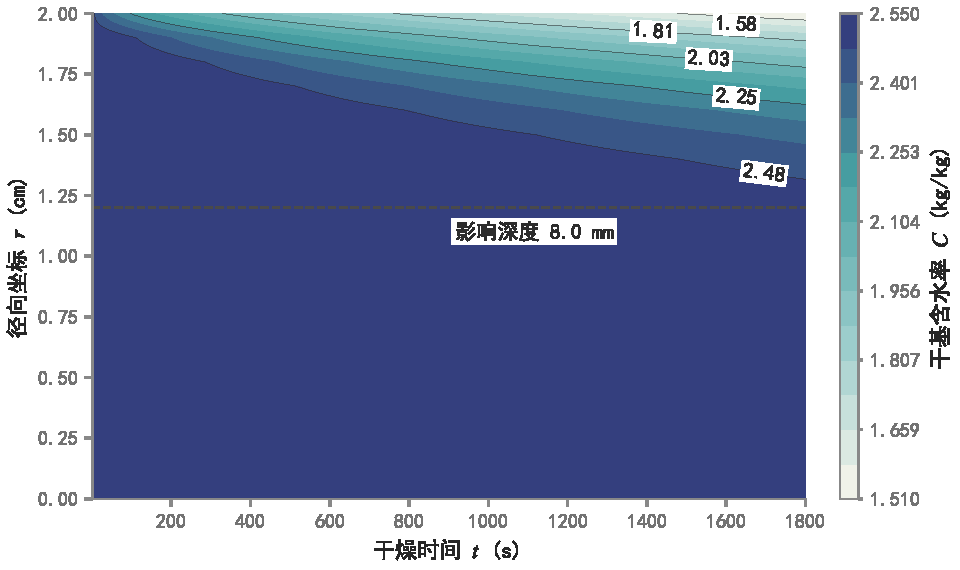
\includegraphics[width=0.9\textwidth,height=0.8\textheight,keepaspectratio]{../figures/fig_q1_field_C.pdf}
  \caption{问题一含水率场分布}
  \label{fig:q1_field_C}
\end{figure}

含水率场的形态与此形成对照。在图~\ref{fig:q1_field_C}~中等值线始终挤在
最外侧，中心大片区域保持初值。$1800$ s 时 $r\le1.0$ cm 处的降幅不足 $0.5\%$，
按干质量加权计最外 $4$ mm 承担了全部失水的 $84.4\%$，而表面已由 $2.5500$ 降到
$1.5103$ kg/kg。这是式~\eqref{eq:D_app2}~给出的扩散系数比热扩散率小
一个半数量级的直接结果，不是数值上的凝滞。

\begin{figure}[!htbp]
  \centering
  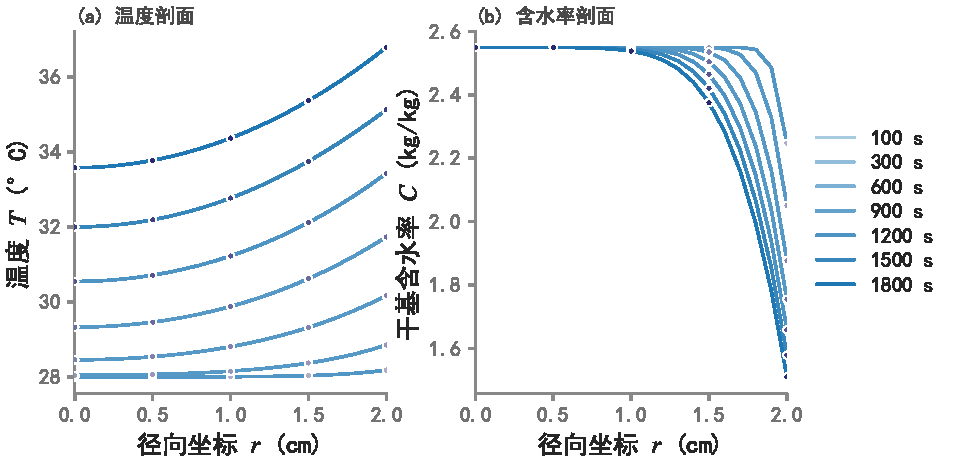
\includegraphics[width=0.9\textwidth,height=0.8\textheight,keepaspectratio]{../figures/fig_q1_profiles.pdf}
  \caption{问题一径向剖面族}
  \label{fig:q1_profiles}
\end{figure}

把两个场按七个制表时刻切成剖面族，可以看得更细
（图~\ref{fig:q1_profiles}，散点标出五个制表半径）。
温度剖面整体抬升、形状相似，属于典型的渗透型加热；
含水率剖面则是根部固定在 $2.55$、只有末端被向下拉的“折线”形态，
干燥前沿尚未离开表层。五个制表半径在 $N=160$ 的网格上对应
$s=0$、$0.0625$、$0.25$、$0.5625$、$1$，恰好落在节点 $i=0,10,40,90,160$ 上，
故下面两张表的数值是节点原值，不含空间插值误差。
\fi

\begin{table}[H]
  \centering
  \caption{问题一各时刻各位置温度（°C）}
  \label{tab:q1_T}
  \begin{tabular}{cccccc}
  \toprule
  时刻 (s) & $r=0$ cm & $r=0.5$ cm & $r=1.0$ cm & $r=1.5$ cm & $r=2.0$ cm \\
  \midrule
  100  & 28.0001 & 28.0004 & 28.0041 & 28.0328 & 28.1802 \\
  300  & 28.0410 & 28.0637 & 28.1516 & 28.3683 & 28.8491 \\
  600  & 28.4538 & 28.5364 & 28.8043 & 29.3162 & 30.1655 \\
  900  & 29.3248 & 29.4587 & 29.8759 & 30.6165 & 31.7306 \\
  1200 & 30.5432 & 30.7102 & 31.2228 & 32.1129 & 33.4279 \\
  1500 & 31.9962 & 32.1871 & 32.7664 & 33.7465 & 35.1204 \\
  1800 & 33.5757 & 33.7723 & 34.3644 & 35.3624 & 36.7857 \\
  \bottomrule
  \end{tabular}
\end{table}

表~\ref{tab:q1_T}~沿半径严格递增、沿时间严格递增，
$100$ s 时中心仅升温 $0.0001$ °C，说明热扰动此时还没有到达轴心。
这些温度有一个已知的偏向需要一并交代：按假设（3）本文未显式建模
汽化潜热引起的表面降温，实际表面温度应略低于表中数值。
第~\ref{sec:validation}~节的灵敏度结果界定了该简化的后果——
对流换热系数变化 $\pm20\%$ 时烘干时长仅改变约 $0.03\%$，
表面热阻并非控制环节，故表面温度的估计偏差不会传导为时长的显著偏差。

\begin{table}[H]
  \centering
  \caption{问题一各时刻各位置水分浓度（kg/kg）}
  \label{tab:q1_C}
  \begin{tabular}{cccccc}
  \toprule
  时刻 (s) & $r=0$ cm & $r=0.5$ cm & $r=1.0$ cm & $r=1.5$ cm & $r=2.0$ cm \\
  \midrule
  100  & 2.5500 & 2.5500 & 2.5500 & 2.5500 & 2.2473 \\
  300  & 2.5500 & 2.5500 & 2.5500 & 2.5492 & 2.0509 \\
  600  & 2.5500 & 2.5500 & 2.5500 & 2.5353 & 1.8770 \\
  900  & 2.5500 & 2.5500 & 2.5497 & 2.5045 & 1.7548 \\
  1200 & 2.5500 & 2.5500 & 2.5482 & 2.4646 & 1.6586 \\
  1500 & 2.5500 & 2.5499 & 2.5445 & 2.4206 & 1.5788 \\
  1800 & 2.5500 & 2.5497 & 2.5383 & 2.3755 & 1.5103 \\
  \bottomrule
  \end{tabular}
\end{table}

含水率一侧的分布则极不均匀。表~\ref{tab:q1_C}~的中心列七个时刻全部
保持 $2.5500$，$r=0.5$ cm 处直到 $1500$ s 才在第四位小数上出现变化，
而表面列已下降 $1.0397$ kg/kg。按式~\eqref{eq:global_balance}~所用的
干质量加权计，$1800$ s 时截面平均含水率为 $2.2936$ kg/kg，
即预热段总共排出初始水分的 $10.06\%$。
两张表并读可以给预热阶段定性：它主要是升温过程，
脱水虽已开始却局限在表层，中心区域尚未启动。
$1800$ s 内每隔 $1$ s、每隔 $0.1$ cm 的完整结果见 \verb|result1.xlsx|，
温度与水分浓度各一张工作表，每表 $1800$ 行 $\times$ $22$ 列。
后文交付文件的列数一律按含时间列的表头长度计，
$22$ 列即一列时间标签加 $0$ 至 $2.0$ cm 共 $21$ 个半径列。

\subsection{热、质推进的尺度分离}

热扰动已贯穿半径而湿分仍局限于表层，故预热的主要作用是升温；完整热湿推进图见附录 B。
\iffalse

\begin{figure}[!htbp]
  \centering
  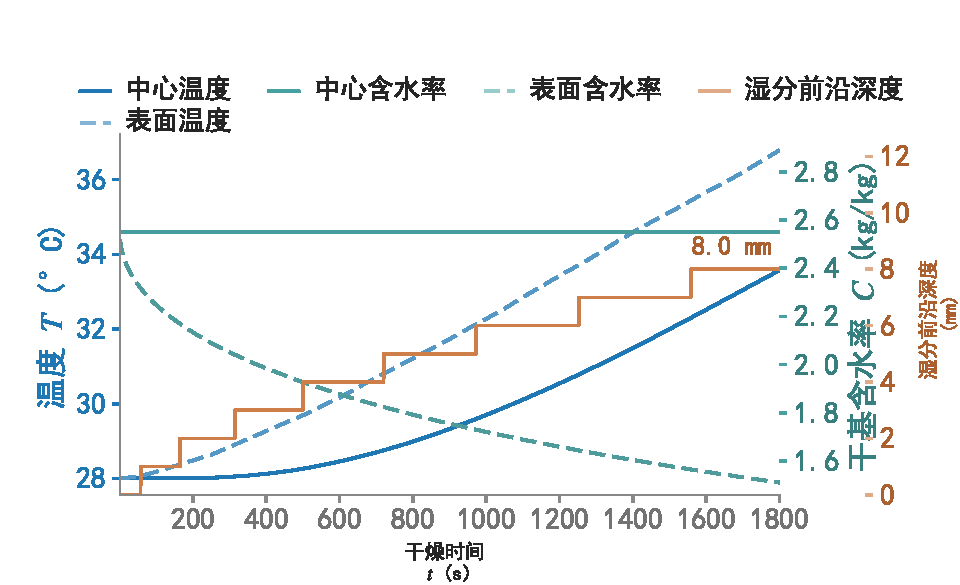
\includegraphics[width=0.9\textwidth,height=0.8\textheight,keepaspectratio]{../figures/fig_q1_penetration.pdf}
  \caption{问题一热湿推进对比}
  \label{fig:q1_penetration}
\end{figure}

热扰动在 $1800$ s 内已贯穿整个半径，而湿扰动只走完不到半个半径
（图~\ref{fig:q1_penetration}~把中心与表面的温度、含水率时程和湿分渗透深度
画在一起）。温度一侧，中心曲线在约 $200$ s 后开始明显抬升，
到 $1800$ s 已跟随表面上升、两条线的间距稳定在 $3$ °C 量级，
即热扰动已走完全程。含水率一侧，表面曲线迅速下落，
中心曲线在整个时窗内是一条水平线。以偏离初值 $1\%$ 为前沿判据，
渗透深度到 $1800$ s 才推进到 $8.0$ mm，约为半径的五分之二，
且其中最外 $4$ mm 就占了失水量的八成以上。

这一对照给预热平衡阶段一个明确的物理定位：题面称之为“预热”是准确的，
该阶段的实质是把冷料整体升温至接近热风温度，脱水只在表层发生。
后续三问中真正决定烘干时长的湿分输运，在这一阶段还没有进入内部。
反过来说，问题二至问题四之所以需要几十小时，也正是因为湿分必须走完
热量在半小时内就走完的那段路程。

\subsection{解析解校验}

\fi
\subsection{解析解校验摘要}
常物性温度方程可由 Bessel--Duhamel 展开独立求解。采用减法变量 $T-T_{\mathrm{air}}$ 后，解析解与有限体积数值解的最大偏差仅 $5.224\times10^{-4}$ °C，说明温度方程及 Robin 边界的实现一致；完整推导和残差图见附录 B。
\iffalse

数值结果的可信度需要一条不依赖本文离散格式的独立通道来支撑。
由于式~\eqref{eq:p1_heat}~在附录 2 闭合下是常系数线性方程、
且与水分方程解耦，可以用特征函数展开配合 Duhamel 叠加求出解析解。
圆柱在对流边界下的瞬态导热本身有成熟的解析处理\upcite{guellal2009cylinder}，
非齐次与混合边界情形则须借助级数重构\upcite{zare2018analytic}，
本文的做法属于后者。

齐次 Robin 特征值问题 $\frac{1}{r}(rX')'+\zeta^2X/R_0^2=0$、$-kX'(R_0)=hX(R_0)$
给出以零阶 Bessel 函数为形状的特征函数与超越特征方程

\begin{equation}
X_n(r)=J_0\!\left(\zeta_n\frac{r}{R_0}\right),
\qquad
\zeta_nJ_1(\zeta_n)=\mathrm{Bi}\,J_0(\zeta_n),
\qquad
\lambda_n=\frac{\alpha\zeta_n^{2}}{R_0^{2}}.
\label{eq:eigen}
\end{equation}

式~\eqref{eq:eigen}~的根须在 $J_1$ 的相邻零点区间内逐个用 Brent 法求解；
若对全部模态使用统一初值迭代，多个模态会收敛到同一根。
本文求得 $\zeta_{1\sim6}=1.41847$、$4.16647$、$7.20848$、$10.30827$、
$13.42716$、$16.55454$，与文献参照值最大偏差 $3.96\times10^{-6}$，
基频衰减率 $\lambda_1=8.4937\times10^{-4}$ 1/s。

关键之处在于不能直接对 $T$ 做叠加。展开系数

\begin{equation}
A_n=\frac{2J_1(\zeta_n)}{\zeta_n\left[J_0^{2}(\zeta_n)+J_1^{2}(\zeta_n)\right]}
\label{eq:An}
\end{equation}

满足 $\sum_nA_nJ_0(\zeta_nr/R_0)=1$，但常数 $1$ 并不满足齐次 Robin 条件，
该展开非一致收敛、$A_n$ 只以 $\zeta_n^{-1/2}$ 衰减。$T_{\mathrm{air}}$ 缓变时的
准稳态响应会把这条慢收敛尾巴永久留在解里：实测偏差卡在 $0.196$ °C，
且仅随模态数 $M$ 以 $1/M$ 下降，增加模态几乎无效。

改令 $\theta(r,t)=T(r,t)-T_{\mathrm{air}}(t)$。$\theta$ 满足齐次 Robin 条件，
方程带源项 $-\dot T_{\mathrm{air}}(t)$，展开为

\begin{equation}
\theta(r,t)=\sum_{n=1}^{M}b_n(t)J_0\!\left(\zeta_n\frac{r}{R_0}\right),
\qquad
\dot b_n=-\lambda_nb_n-A_n\dot T_{\mathrm{air}}(t).
\label{eq:duhamel}
\end{equation}

附件 1 在 $60$ s 间隔上分段线性，故每段内 $\dot T_{\mathrm{air}}$ 为常数，
式~\eqref{eq:duhamel}~可逐段精确积分：

\begin{equation}
b_n^{j+1}=b_n^{j}\mathrm{e}^{-\lambda_n\Delta}
-A_n\frac{T_{\mathrm{air}}^{j+1}-T_{\mathrm{air}}^{j}}{\Delta}
\cdot\frac{1-\mathrm{e}^{-\lambda_n\Delta}}{\lambda_n},
\qquad
T=T_{\mathrm{air}}(t)+\theta,
\label{eq:bn_exact}
\end{equation}

其中 $\Delta=60$ s。减法形式下常数部分由前导项 $T_{\mathrm{air}}(t)$ 承担，
残余级数只需展开满足齐次边界的 $\theta$，系数以 $n^{-5/2}$ 衰减。

\begin{figure}[!htbp]
  \centering
  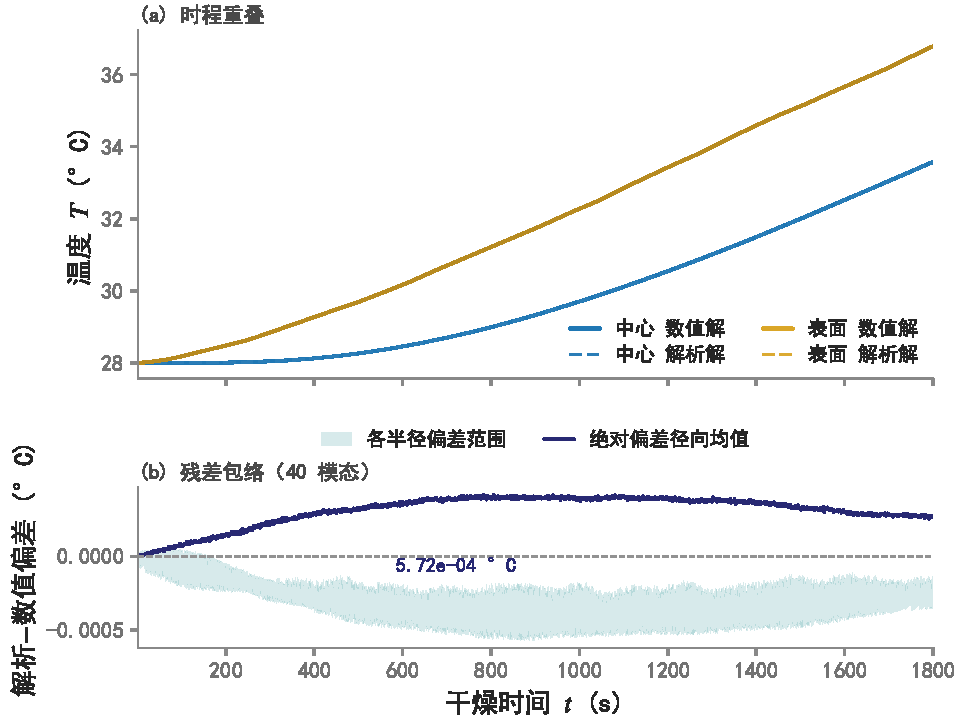
\includegraphics[width=0.9\textwidth,height=0.8\textheight,keepaspectratio]{../figures/fig_q1_analytic_val.pdf}
  \caption{解析解与数值解对比}
  \label{fig:q1_analytic_val}
\end{figure}

两条求解路径在全时窗、全半径上给出同一条温度曲线，最大偏差为
$5.224\times10^{-4}$ °C（图~\ref{fig:q1_analytic_val}~及其残差面板）。
该偏差取自 $M=40$ 个模态的截断；按 $M=6$、$12$、$20$、$40$ 逐档加模态，
偏差依次为 $1.838\times10^{-3}$、$5.565\times10^{-4}$、$5.257\times10^{-4}$、
$5.224\times10^{-4}$ °C，末两档只差 $3.3\times10^{-6}$ °C，
说明级数在 $M=40$ 处已收敛，残余偏差不来自截断。
它来自数值解自身的离散误差地板：把网格加密到 $N=640$、时间步减到 $0.05$ s 后，
同一模态数下偏差降到 $9.781\times10^{-5}$ °C，
即偏差随离散加密而下降、随模态数增加而不再变化，
两条求解路径在此精度内给出同一个解。
需要说明这一校验的范围：解析解与数值解共用同一组常物性和同一个 Robin 边界，
两者相符检验的是有限体积格式是否正确求解了该方程，属实现层面的独立校核，
不构成对模型物理设定（如不含潜热）的验证。
校验还有一处值得指出：附件 1 给出 $T_{\mathrm{air}}(0)=28.000000$ °C
与初始温度精确相等，故式~\eqref{eq:duhamel}~的初值 $b_n(0)\equiv0$，
本次比对检验的是完全由边界驱动的响应，不含初值瞬态带来的平凡吻合。
\fi
